\section{第4讲\quad 计数问题}

\item {
    【几何计数·三角形】
    下图中, 共有\underline{\hbox to 20mm{}}个三角形.
    \begin{figure}[H] 
        \centering
        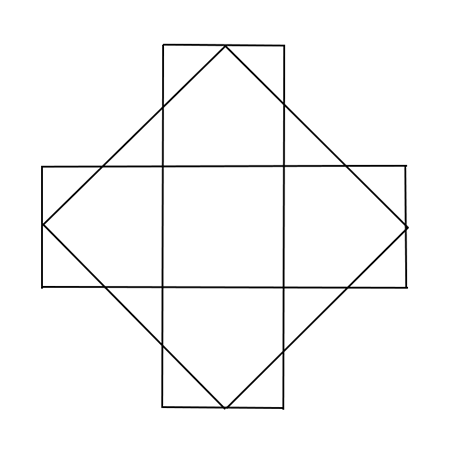
\includegraphics[width=0.3\textwidth]{./pics/Chapter_4/12.png}
    \end{figure}
    \ifshowSolution 
        \fangsong\zihao{5}\textcolor{blue}{
            正解: \\
            小三角形:12个;大三角形:4个。共16个。
        }
    \else
        \vspace{1cm}
    \fi
    % 2021; 迎春杯三年级真题.pdf ; 16
}

\item {
    【几何计数·三角形】
    如图中共能数出\underline{\hbox to 20mm{}}个三角形.
    \begin{figure}[H] 
        \centering
        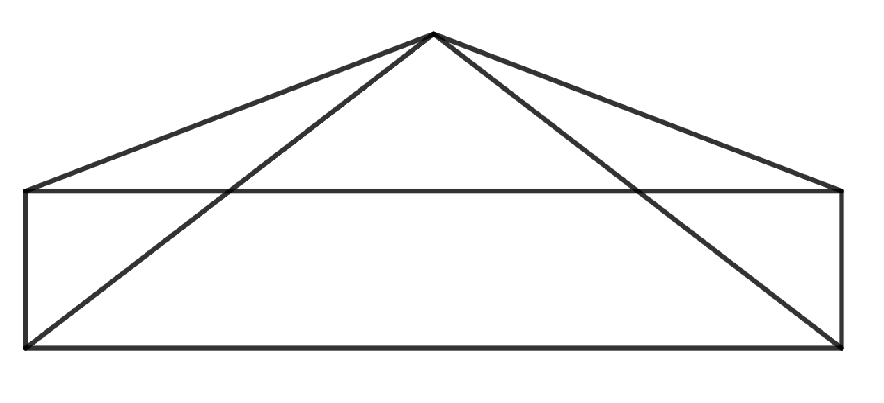
\includegraphics[width=0.4\textwidth]{./pics/Chapter_4/2015_1.png}
    \end{figure}
    \ifshowSolution 
        \fangsong\zihao{5}\textcolor{blue}{
            正解: \\
            1部分组成的三角形:5个;\\
            2部分组成的三角形:5个;\\
            3部分组成的三角形:1个。\\
            共11个。
        }
    \else
        \vspace{1cm}
    \fi
    % 2015年“迎春杯”数学花园探秘科普活动试卷(小中组决赛c卷).doc ; 11
}

\item {
    【几何计数·三角形】
    数一数, 如图中共有\underline{\hbox to 20mm{}}个三角形.
    \begin{figure}[H] 
        \centering
        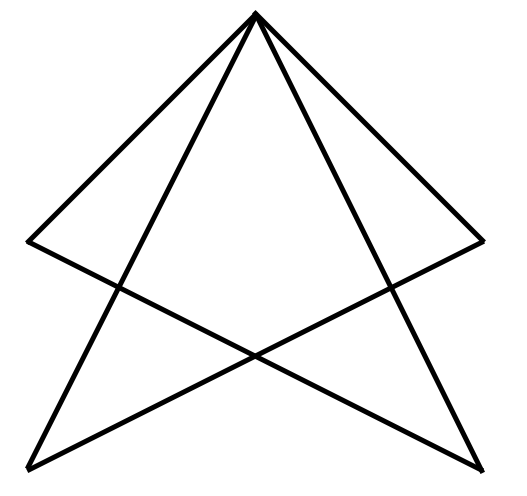
\includegraphics[width=0.2\textwidth]{./pics/Chapter_4/2015_2.png}
    \end{figure}
    \ifshowSolution 
        \fangsong\zihao{5}\textcolor{blue}{
            正解: \\
            1部分组成的三角形:4个;\\
            2部分组成的三角形:2个;\\
            3部分组成的三角形:2个。\\
            共8个。
        }
    \else
        \vspace{1cm}
    \fi
    % 2015年“迎春杯”数学花园探秘科普活动试卷(四年级初赛b卷).doc ; 8
}

\item {
    【几何计数】
    下图是由 ``开罗五边形'' 组成的拼接图, 图中的每个五边形的形状大小完全相同, 观察图形并确定下右图中的图形在下左图中共出现了\underline{\hbox to 20mm{}}次. (右图图形可以旋转观察)
    \begin{figure}[H] 
        \centering
        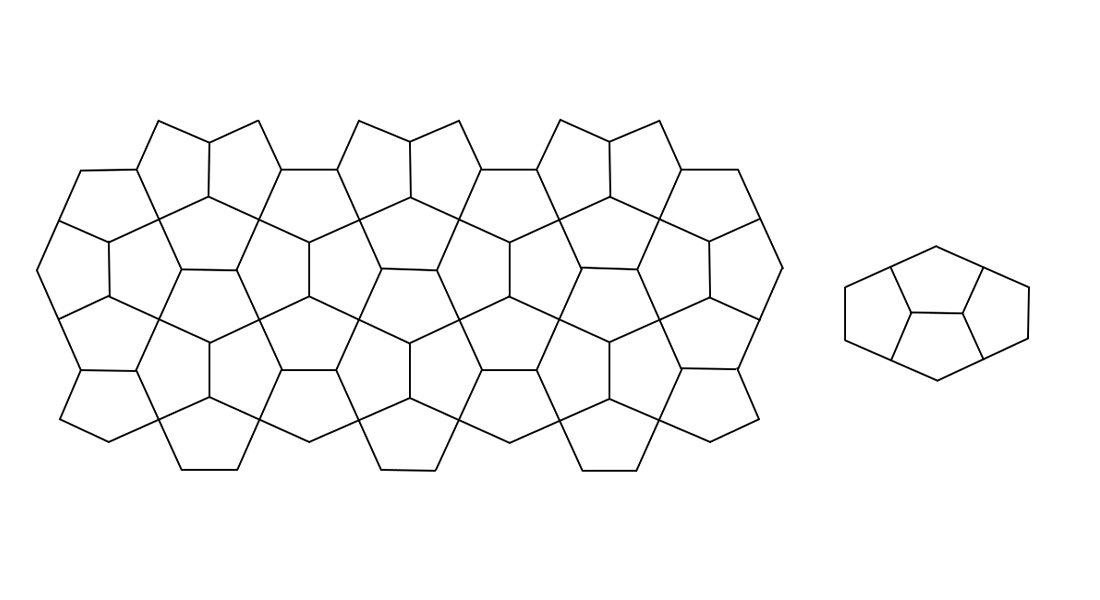
\includegraphics[width=0.5\textwidth]{./pics/Chapter_4/8.png}
    \end{figure}
    \ifshowSolution 
        \fangsong\zihao{5}\textcolor{blue}{
            正解: \\
            横向:5个;纵向:7个。
            共12个。
        }
    \else
        \vspace{1cm}
    \fi
    % 迎春杯三年级2022-试卷.pdf ;  12
}

\item {
    【几何计数·正六边形】
    右图中, 共有\underline{\hbox to 20mm{}}个正六边形.
    \begin{figure}[H] 
        \centering
        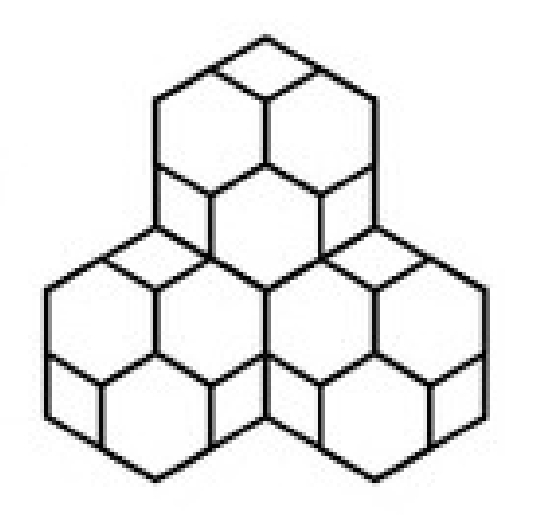
\includegraphics[width=0.2\textwidth]{./pics/Chapter_4/14.png}
    \end{figure}
    \ifshowSolution 
        \fangsong\zihao{5}\textcolor{blue}{
            正解: \\
            小正六边形:9个;大正六边形:3个。
            共12个。
        }
    \else
        \vspace{1cm}
    \fi
    % 2021 ;  迎春杯四年级真题.pdf ;  12
}

\item {
    【几何计数·梯形】
    如图中共有\underline{\hbox to 20mm{}}个梯形.
    \begin{figure}[H] 
        \centering
        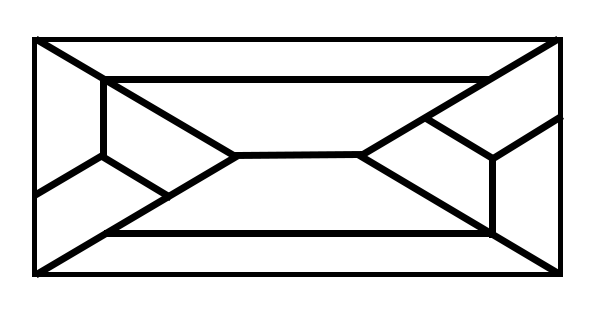
\includegraphics[width=0.3\textwidth]{./pics/Chapter_4/2016_1.png}
    \end{figure}
    \ifshowSolution 
        \fangsong\zihao{5}\textcolor{blue}{
            正解: \\
            1部分组成的梯形:10个;\\
            2部分组成的梯形:2个。\\
            共12个。
        }
    \else
        \vspace{1cm}
    \fi
    % 2016年“迎春杯”数学花园探秘网试试卷(四年级).doc ; 12
}

\item {
    【几何计数·平行四边形】
    如图中共有\underline{\hbox to 20mm{}}个平行四边形.
    \begin{figure}[H] 
        \centering
        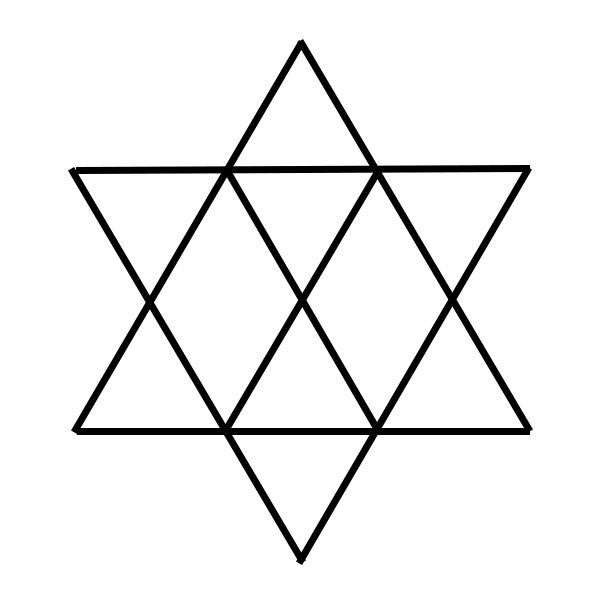
\includegraphics[width=0.2\textwidth]{./pics/Chapter_4/2017_1.png}
    \end{figure}
    \ifshowSolution 
        \fangsong\zihao{5}\textcolor{blue}{
            正解: \\
            方法1\\
            1部分组成:2个;\\
            2部分组成:2个;\\
            3部分组成:8个;\\
            6部分组成:3个。\\
            共15个。\\\\
            方法2(平行线)\\
            \begin{figure}[H] 
                \centering
                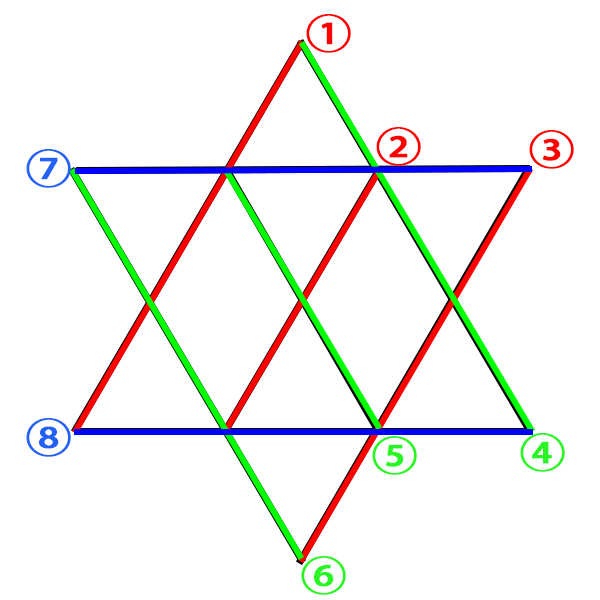
\includegraphics[width=0.2\textwidth]{./pics/Chapter_4/seikai_2017_1.png}
            \end{figure}
            \textcircled{1}\textcircled{2}: 4个;\\
            \textcircled{1}\textcircled{3}: 4个;\\
            \textcircled{2}\textcircled{3}: 3个;\\
            \textcircled{7}\textcircled{8}: 3个;\\
            共15个。
        }
    \else
        \vspace{1cm}
    \fi
    % 2017年“迎春杯”数学花园探秘科普活动试卷(小中组决赛a卷).doc ; 15
}

\item {
    【数量关系】
    如右图, 小鱼老师在为圣诞树准备装饰物, 每个树顶需要放一颗幸运星每一层树的两侧需要各放 1 个许愿球, 一共 3 层, 小鱼老师数了数, 许愿球比幸运星多 40 个, 那么, 小鱼老师装饰了\underline{\hbox to 20mm{}}棵圣诞树.
    \begin{figure}[H] 
        \centering
        
\includegraphics[width=0.2\textwidth]{./pics/Chapter_4/13.png}
    \end{figure}
    \ifshowSolution
        \fangsong\zihao{5}\textcolor{blue}{
            \\正解: \\
            一棵圣诞树有1个幸运星,6个许愿球;许愿球比幸运星多5个。\\
            $40\div 5 = 8$棵。
        }
    \else
        \vspace{1cm}
    \fi
    % 2021; 迎春杯三年级真题.pdf ;  8
}

\item {
    【图形拼接】
    在平面上用长度为6厘米的牙签棒摆正方形, 摆出一个长为6厘米的正方形需要4根牙签棒, 摆出5个这样的正方形至少需要\underline{\hbox to 20mm{}}根牙签棒. 
    \ifshowSolution 
        \fangsong\zihao{5}\textcolor{blue}{
            \\正解: \\
            \begin{figure}[H] 
                \centering
                
\includegraphics[width=0.2\textwidth]{./pics/Chapter_4/seikai_2016_3d.png}
            \end{figure}
            至少需要15根。
        }
    \else
        \vspace{1cm}
    \fi
    % 2016年“迎春杯”数学花园探秘初赛试卷(三年级d卷).doc ; 15
}

\item {
    【图形拼接】
    丽丽想用大小为 $1\times 1, 2\times 2, 3\times 3$的三种正方形拼成下图所示的领奖台(图中每个小正方形的边长为1),所用正方形的面积总和为 15,且拼接过程中不可重叠,每种正方形数量不限(可以不用).共有\underline{\hbox to 20mm{}}种不同的拼接方法.(正方形的摆放位置或数量不同都算不同的拼法)
    \begin{figure}[H] 
        \centering
        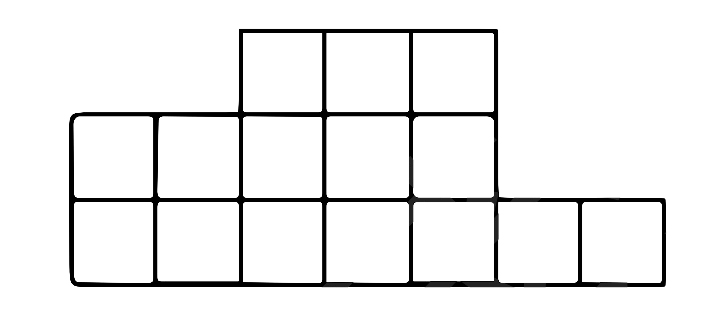
\includegraphics[width=0.4\textwidth]{./pics/Chapter_4/9.png}
    \end{figure}
    \ifshowSolution 
        \fangsong\zihao{5}\textcolor{blue}{
            正解: \\
            列表枚举。\\
            \begin{tabular}{|c|c|c|c|}
                \hline
                $3\times 3$ & $2\times 2$ & $1\times 1$ & 摆法 \\
                \hline
                1 & 1 & 2 & 1 \\
                1 & 0 & 6 & 1 \\
                0 & 2 & 7 & 6 \\
                0 & 1 & 11 & 6 \\
                0 & 0 & 15 & 1 \\
                \hline
            \end{tabular} \\
            共15种。
        }
    \else
        \vspace{1cm}
    \fi
    % 迎春杯三年级2022-试卷.pdf ;  15
}

\item {
    【体育比赛·枚举】
    老师手中有4张牌, 按照``甲、乙、甲、乙''的顺序分发。如果这4张牌的点数分别是 1、2、3、4, 并且在整个过程中(包括最终), 甲手中牌的点数之和一直比乙大, 那么, 满足要求的分发顺序共有\underline{\hbox to 20mm{}}种.
    \ifshowSolution
        \fangsong\zihao{5}\textcolor{blue}{
            \\正解: 符合条件的比分树形图(甲:乙)如下。\\
            \begin{forest}
                [0:0
                    [2:0
                        [2:1
                            [2+4:1
                                [2+4:1+3]
                            ]
                        ]
                    ]
                    [3:0
                        [3:1
                            [3+4:1
                                [3+4:1+2]
                            ]
                        ]
                        [3:2
                            [3+4:2
                                [3+4:2+1]
                            ]
                        ]
                    ]
                    [4:0
                        [4:1
                            [4+2:1
                                [4+2:1+3]
                            ]
                            [4+3:1
                                [4+3:1+2]
                            ]
                        ]
                        [4:2
                            [4+3:2
                                [4+3:2+1]
                            ]
                        ]
                        [4:3
                            [4+2:3
                                [4+2:3+1]
                            ]
                        ]
                    ]
                ]
            \end{forest}
            \\共7种。
        }
    \else
        \vspace{1cm}
    \fi
    % 迎春杯四年级2022-试卷.pdf ;  7
}

\item {
    【染色覆盖】
    如图, 一个$2\times 2\times 2$的正方体六个面已经被染成了不同的六种颜色. 现将其分成4个$2\times 1\times 1$的小长方体, 共有\underline{\hbox to 20mm{}}种不同分法.
    \begin{figure}[H] 
        \centering
        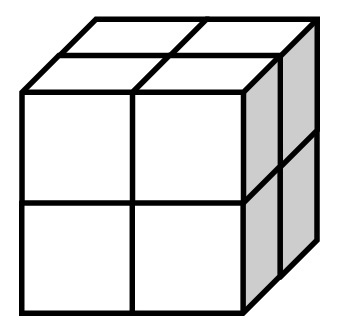
\includegraphics[width=0.2\textwidth]{./pics/Chapter_4/15.png}
    \end{figure}
    \ifshowSolution 
        \fangsong\zihao{5}\textcolor{blue}{
            正解: \\
            4个小长方体同向:3种;\\
            2个同向 + 2个异向:6种,\\
            共9种。
        }
    \else
        \vspace{1cm}
    \fi
    % 2020数学花园探秘笔试小中决赛D卷.doc ; 9
}

\item {
    【立体图形·组合】
    图\textcircled{3}是由6个图\textcircled{1}这样的模块拼成的, 如果最底层已经给定两块的位置 (如图\textcircled{2}), 那么剩下部分一共有\underline{\hbox to 20mm{}}种不同的拼法.
    \begin{figure}[H] 
        \centering
        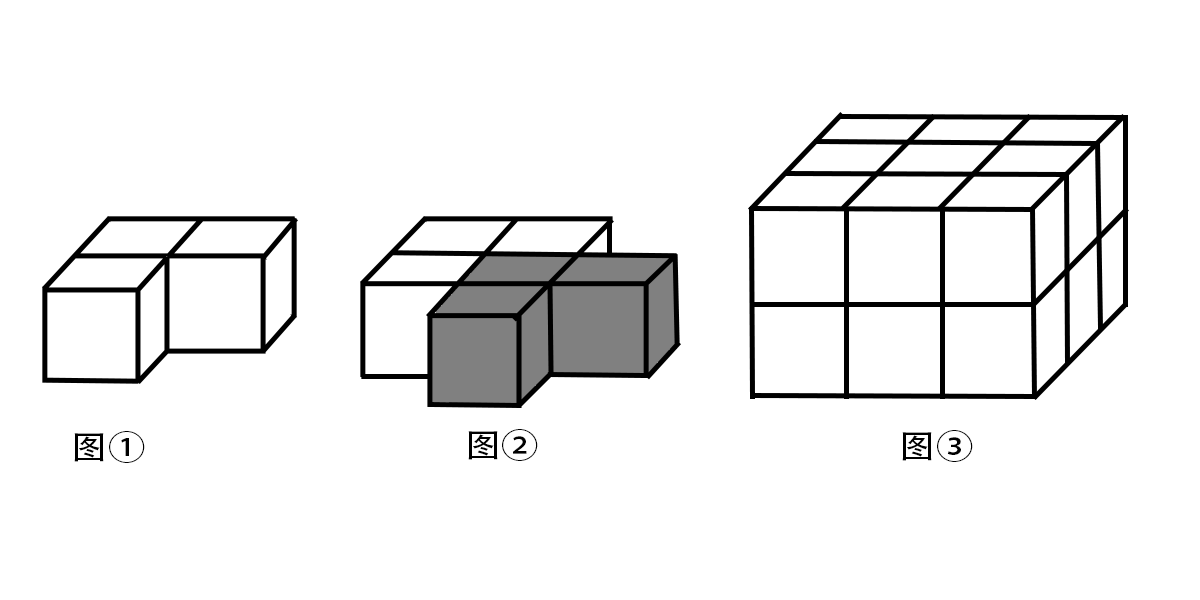
\includegraphics[width=0.5\textwidth]{./pics/Chapter_4/2016_2.png}
    \end{figure}
    \ifshowSolution 
        \fangsong\zihao{5}\textcolor{blue}{
            正解: \\
            共2种不同拼法,如下:\\
            \begin{figure}[H] 
                \centering
                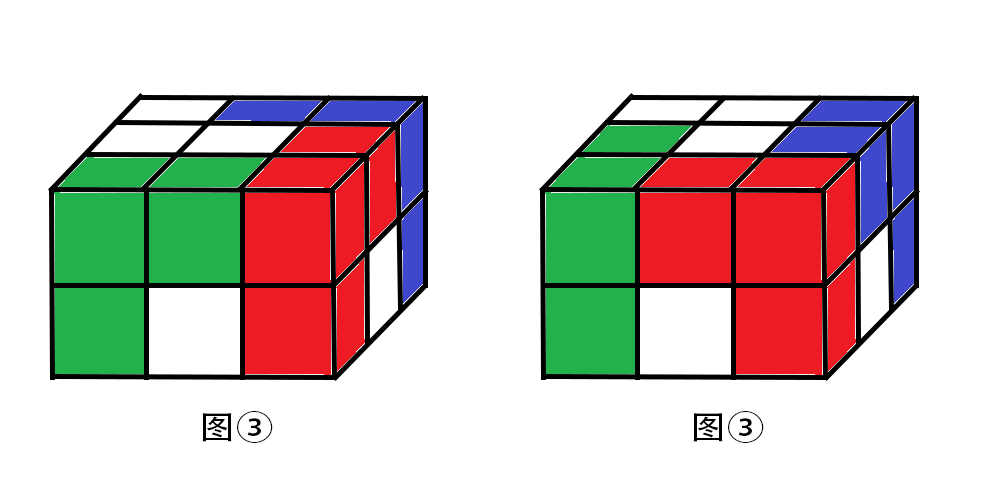
\includegraphics[width=0.5\textwidth]{./pics/Chapter_4/seikai_2016_2.png}
            \end{figure}
        }
    \else
        \vspace{1cm}
    \fi
    % 2016年“迎春杯”数学花园探秘决赛试卷(小中组c卷).doc ; 2
}

\item {
    【数列·找规律】
    有一颗神奇的树上长了58个果子, 第一天会有1个果子从树上掉落. 从第二天起, 每天掉落的果子数量比前一天多1个, 但如果某天树上的果子数量少于这一天本应该掉落的数量时, 那么这一天它又重新从掉落1颗果子开始. 按原规律进行新的一轮. 如此继续. 那么第\underline{\hbox to 20mm{}}天树上的果子会掉光.
    \ifshowSolution 
        \fangsong\zihao{5}\textcolor{blue}{
            \\正解: \\
            前10天,掉落果子的总数:$1+2+\cdots +10 = 55$,还剩 $58-55=3$ 个;\\
            第11天,掉落1个,还剩2个;\\
            第12天,掉落2个,还剩0个。
        }
    \else
        \vspace{1cm}
    \fi
    % 2016年“迎春杯”数学花园探秘初赛试卷(四年级d卷).doc ; 12
}


\item {
    【几何计数·找规律】
    如图所示, 从正三角形的边作一个正方形, 再用与正三角形不相邻的正方形一边做一个正五边形, 再从与正方形不相邻的正五边形一边作一个正六边形, 继续以相同的方式再作一个正七边形, 依序再作一个正八边形, 这样形成了一个多边形, 请问这个多边形有\underline{\hbox to 20mm{}}个边. 
    \begin{figure}[H] 
        \centering
        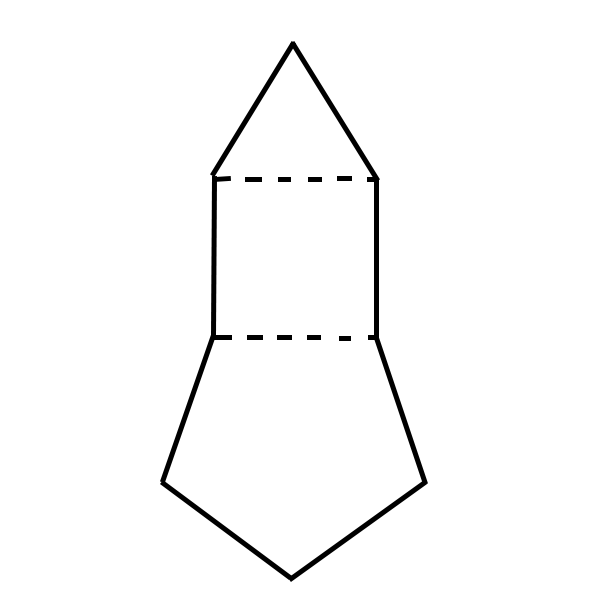
\includegraphics[width=0.3\textwidth]{./pics/Chapter_4/2015_3.png}
    \end{figure}
    \ifshowSolution 
        \fangsong\zihao{5}\textcolor{blue}{
            \\正解: \\
            \begin{tabular}{|c|c|c|c|}
                \hline
                $图形$ & $边数$ \\
                \hline
                正三角形 & 3 \\
                正三角形+正方形 & 3+2 \\
                正三角形+正方形+正五边形 & 3+2+3 \\
                $\cdots$ & $\cdots$ \\
                正三角形+正方形+$\cdots$+正八边形 & 3+2+3+4+5+6=23 \\
                \hline
            \end{tabular} \\
        }
    \else
        \vspace{1cm}
    \fi
    % 2015年“迎春杯”数学花园探秘科普活动试卷(三年级初赛b卷).doc ; 23
}

\item {
    【组合计数】
    如图所示, 一个圆形托盘上放着三个相同的盘子, 笑笑只将7个相同的苹果放在这一个盘子中, 每个盘子中至少要放一个. 那么笑笑有\underline{\hbox to 20mm{}}种放苹果的方法. (托盘旋转后相同的算同一种情况)
    \begin{figure}[H] 
        \centering
        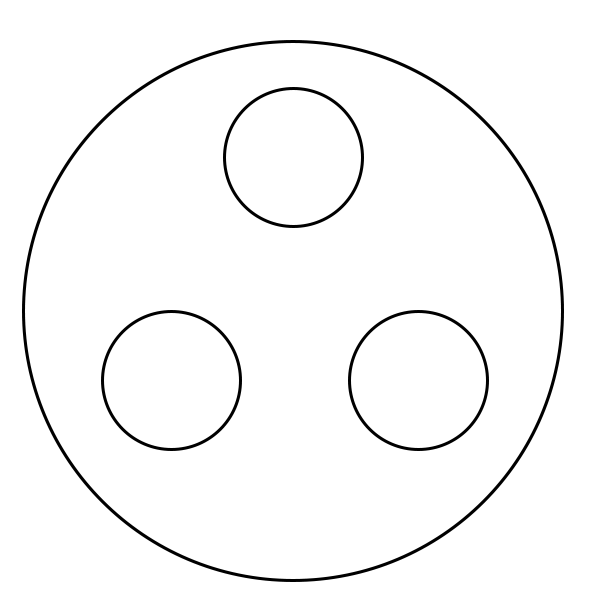
\includegraphics[width=0.2\textwidth]{./pics/Chapter_4/2015_4.png}
    \end{figure}
    \ifshowSolution 
        \fangsong\zihao{5}\textcolor{blue}{
            \\正解: 先将7个苹果分为3份,再摆放。\\
            \begin{tabular}{|c|c|c|c|}
                \hline
                $分法$ & $摆法$ \\
                \hline
                1+1+5 & 1 \\
                1+2+4 & 2 \\
                1+3+3 & 1 \\
                2+2+3 & 1 \\
                \hline
            \end{tabular} \\
            共5种方法。
        }
    \else
        \vspace{1cm}
    \fi
    % 2015年“迎春杯”数学花园探秘科普活动试卷(三年级初赛a卷).doc ; 5
}

\item {
    【几何计数·排列组合】
    用4种不同的颜色来涂正四面体(如图,每个面都是完全相同的正三角形)的4个面,使不同的面涂有不同的颜色,共有\underline{\hbox to 20mm{}}种不同的涂法.(将正四面体任意旋转后仍然不同的涂色法,才被认为是不同的).
    \begin{figure}[H] 
        \centering
        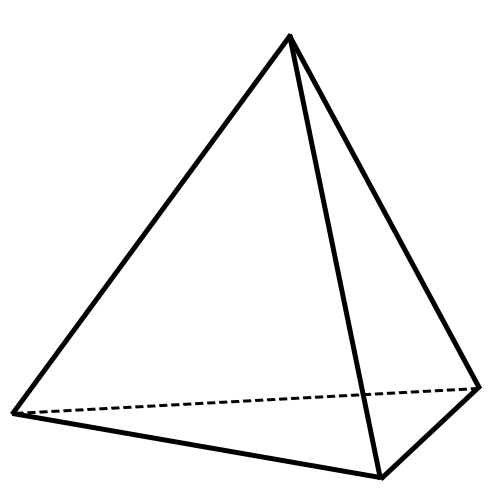
\includegraphics[width=0.2\textwidth]{./pics/Chapter_4/2010_1.png}
    \end{figure}
    \ifshowSolution 
        \fangsong\zihao{5}\textcolor{blue}{
            \\正解: 用A,B,C,D代表4种颜色. 先将底面涂为D色,则3个侧面有2种涂法(俯视图顺时针视角):ABC, ACB.\\
            \begin{figure}[H] 
                \centering
                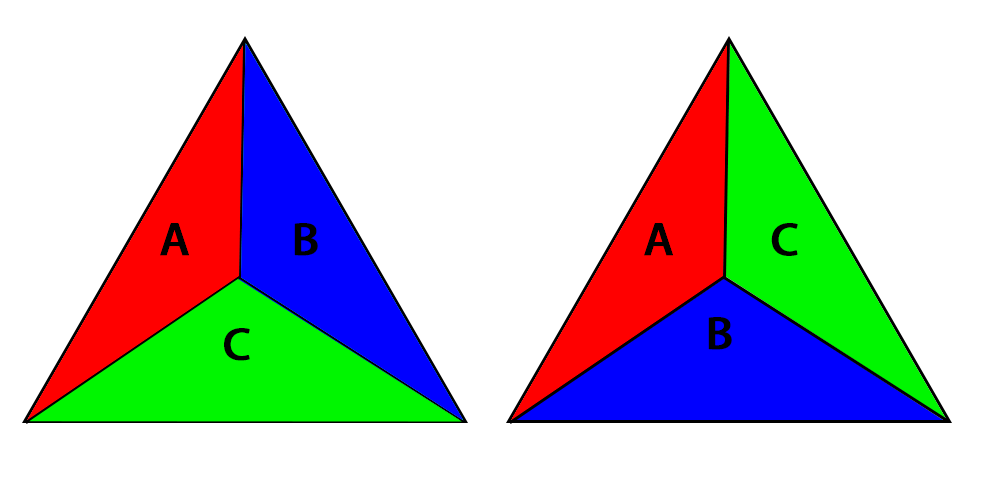
\includegraphics[width=0.3\textwidth]{./pics/Chapter_4/seikai_2010_1.png}
            \end{figure}
        }
    \else
        \vspace{1cm}
    \fi
    % 2010年“迎春杯”数学解题能力展示复赛试卷(小中组).doc ; 2
}

\item {
    【字典排序】
    植物射手有豌豆射手, 双重射手、三重射手、寒冰射手、双向射手、豌豆荚6种. 种植一株该种射手所需要的阳光依次为100、200、300、150、125、125. 菲菲种了10株植物射手共花费2500阳光, 她的种法有\underline{\hbox to 20mm{}}种不同的可能.  (例如, 7株三重射手 + 1株寒冰射手 + 1株豌豆荚, 是符合要求的一种可能. )
    \ifshowSolution 
        \fangsong\zihao{5}\textcolor{blue}{
            \\正解: 表格枚举。\\
            \begin{tabular}{|c|c|c|c|c|c|c|}
                \hline
                组合\textbackslash 植物 & 三重300 & 双重200 & 寒冰150 & 双向125 & 豌豆荚125 & 豌豆100 \\
                \hline
                \textcircled{1}&7&1&&&&2 \\
                \textcircled{2}&7&&2&&&1 \\
                \textcircled{3}&7&&1&2&& \\
                \textcircled{4}&7&&1&1&1& \\
                \textcircled{5}&7&&1&&2& \\
                \textcircled{6}&6&3&&&&1 \\
                \textcircled{7}&6&2&2&&& \\
                \textcircled{8}&5&5&&&& \\
                \hline
            \end{tabular} \\
            共8种不同的可能。
        }
    \else
        \vspace{1cm}
    \fi
    % 2015年“迎春杯”数学花园探秘网试试卷(四年级).doc ; 8
}

\item {
    【分类计数】
    用4种不同颜色给圆圈涂色 (4种颜色可以不全用). 要求有线直接相连的两个圆圈的颜色不同. 则共有\underline{\hbox to 20mm{}}种不同的涂色方法.
    \begin{figure}[H] 
        \centering
        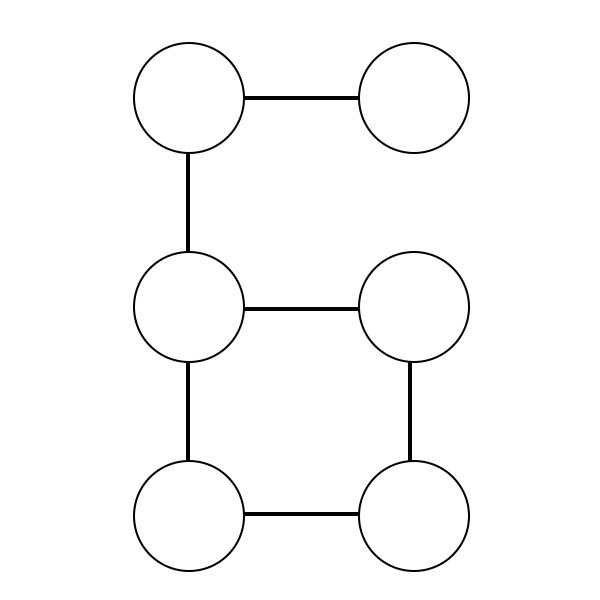
\includegraphics[width=0.2\textwidth]{./pics/Chapter_4/2016_3.png}
    \end{figure}
    \ifshowSolution 
        \fangsong\zihao{5}\textcolor{blue}{
            \\正解: 从1到6给圆圈编号。\\
            \begin{figure}[H] 
                \centering
                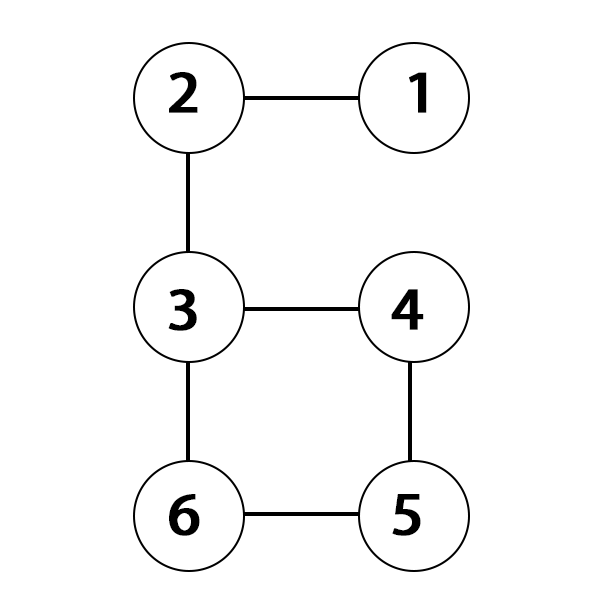
\includegraphics[width=0.2\textwidth]{./pics/Chapter_4/seikai_2016_3.png}
            \end{figure}
            因为4,6号颜色的异同会影响3,5号颜色的选择,所以将4,6分为一组,根据其颜色是否相同讨论。\\
            (1)4,6同色,有4种选择。\\
            3号:3种选择;\\
            2号:3种选择;\\
            1号:3种选择;\\
            5号:3种选择;\\
            所以,有 $4\times 3\times 3\times 3\times 3=324$种涂色方法。\\
            (2)4,6异色,有$4\times 3=12$种选择。\\
            3号:2种选择;\\
            2号:3种选择;\\
            1号:3种选择;\\
            5号:2种选择;\\
            所以,有 $12\times 2\times 3\times 3\times 2=432$种涂色方法。\\
            一共有 $324+432=756$种不同的涂法.
        }
    \else
        \vspace{1cm}
    \fi
    % 2016年“迎春杯”数学花园探秘初赛试卷(四年级c卷).doc ; 756
}

\item {
    【排列组合·分类计数】
    如图, 甲、乙两人从A沿最短路线走到B, 两人所走路线不出现交叉(除A、B两点外没有其它公共点)的走法共有\underline{\hbox to 20mm{}}种. 
    \begin{figure}[H] 
        \centering
        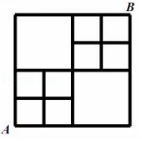
\includegraphics[width=0.2\textwidth]{./pics/Chapter_4/2016_4.png}
    \end{figure}
    \ifshowSolution 
        \fangsong\zihao{5}\textcolor{blue}{
            \\正解: \\
            \begin{figure}[H] 
                \centering
                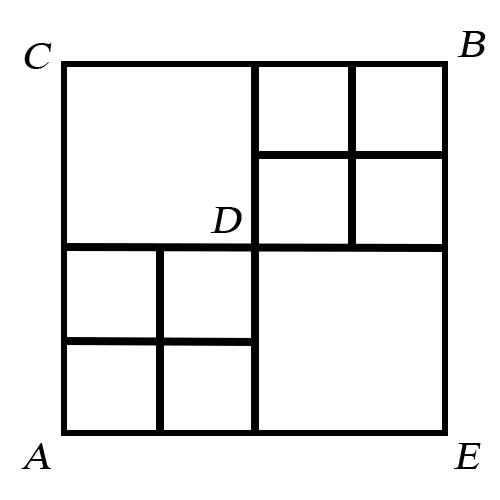
\includegraphics[width=0.2\textwidth]{./pics/Chapter_4/seikai_2016_4.png}
            \end{figure}
            从A走到B,必然要经过C,D,E其中一点。以甲经过哪个点分类讨论。\\
            (1)甲经过C点,有1种走法。\\
            乙:A->D->B,有9种走法;\\
            A->E->B,有1种走法;\\
            (2)甲经过E点,与(1)类似,有10种走法。\\
            (3)甲经过D点,两人有18种走法。\\
            综上,一共有38种走法.
        }
    \else
        \vspace{1cm}
    \fi
    % 2016年“迎春杯”数学花园探秘初赛试卷(四年级a卷).doc ; 38
}

%%%%%%%%%%%%%%%%%%%%%%%%%%%%%
% \item {如图所示, 墙上挂着6件礼物, 分成两列, 每列必须从下往上依次取走。现在有6位同学, 身高分别为 100、120、140、160、180、200厘米.每人只能拿到最多比自己身高高 100 厘米处的礼物.现在6位同学排成一列拿取礼物.为了让每人都能拿到一件礼物, 有\underline{\hbox to 20mm{}}种符合要求的排队方式.
%     \begin{figure}[H] 
%         \centering
%         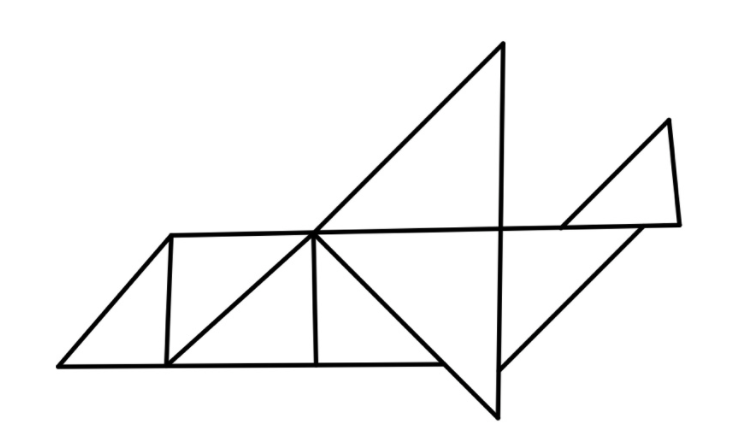
\includegraphics[width=0.5\textwidth]{./pics/Chapter_4/3.png}
%     \end{figure}
%     % 2025数学花园探秘笔试小中年级决赛C卷(解析版).pdf; 40
% }

% \item {如图, 2x3的棋盘上由6个单位正方形构成, 棋盘上共有12 个格点, 甲、乙、丙、丁11.
% 四人站在其中四个格点上, 若任意两人处于同一横线或竖线则认为可相互看见。
% 甲说:我可以看见你们所有人。
% 乙说:我一个人也看不到。
% 丙说:我只能看到一个人。
% 丁说:我们四人所在格点连成四边形面积为3, 且任意3人所在格点组成的三角形面积都不为整数。
% 已知四人中看见人数最多(其他人看见的人数都比他看见的少)的那个人说了假话, 其他人都说了真话, 那么这4人有\underline{\hbox to 20mm{}}种不同的站法.
%     \begin{figure}[H] 
%         \centering
%         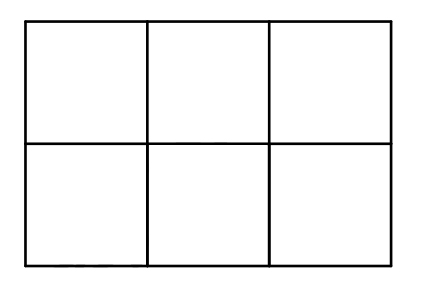
\includegraphics[width=0.5\textwidth]{./pics/Chapter_4/1.png}
%     \end{figure}
%     % 2025数学花园探秘笔试小中年级决赛C卷(解析版).pdf ; 8
% }

% \item {将1、2、3、4、5、6、7、8这八个数字分别填到一个固定好的正方体的八个顶点上, 要求同一条棱上的两个数之和小于12, 那么共有\underline{\hbox to 20mm{}}种不同的填法.
%     % 2024数学花园探秘笔试小中年级夏季决赛C卷(B5试卷版).pdf ;  
% }

% \item {右图已固定, 请将1、2、3、4各两个分别填入八个圆圈中, 使得阴影圆圈中的数比它两边相邻的白色圆圈中的数都大;那么不同的填法共有\underline{\hbox to 20mm{}}种.
%     \begin{figure}[H] 
%         \centering
%         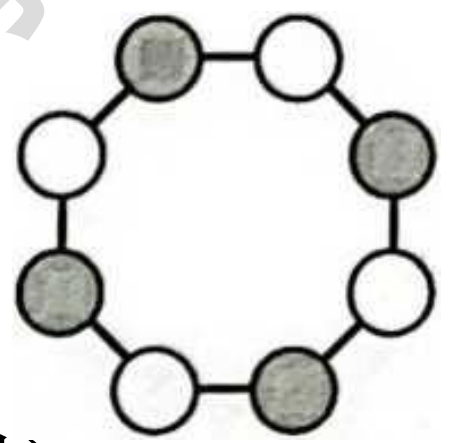
\includegraphics[width=0.5\textwidth]{./pics/Chapter_4/6.png}
%     \end{figure}
%     % 2023YCB初赛真题答案小中.pdf ; 44
% }

% \item {右图中共能数出\underline{\hbox to 20mm{}}个 三角形.
%     \begin{figure}[H] 
%         \centering
%         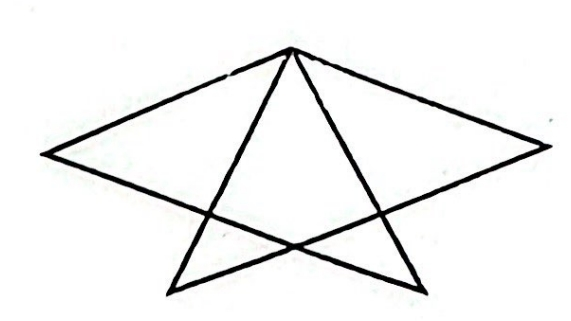
\includegraphics[width=0.5\textwidth]{./pics/Chapter_4/7.png}
%     \end{figure}
%     % 2023; YCB第40届小中组试卷答案.pdf ; 8
% }

% \item {图中, 三角形共有\underline{\hbox to 20mm{}}个.
%     \begin{figure}[H] 
%         \centering
%         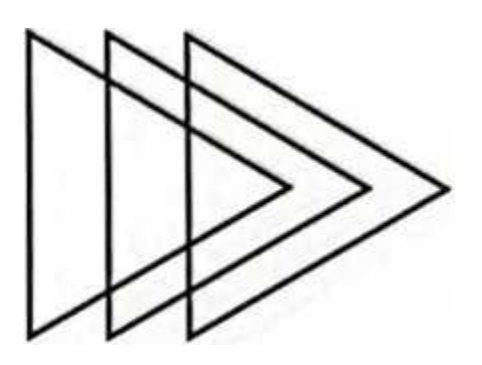
\includegraphics[width=0.5\textwidth]{./pics/Chapter_4/5.png}
%     \end{figure}
%     % 2023YCB初赛真题答案小中.pdf ;  6
% }

% \item {如图, 在正方体的一些顶点处各有一只蚂蚁, 它们的爬行速度相同且只能沿着正方体的棱爬行, 在棱上爬行到达下一个顶点前不能回头, 且从未有任两只蚂蚁相遇.\\
%     (1)如果在 A、B 处各有一只蚂蚁, 每只蚂蚁各爬行1条棱,共有\underline{\hbox to 20mm{}}种不同的爬行情况.\\
%     (2)如果在 A、C、F 处各有一只蚂蚁, 每只蚂蚁各爬行2条棱, 
%     一共有 \underline{\hbox to 20mm{}} 种不同的爬行情况.
%     \begin{figure}[H] 
%         \centering
%         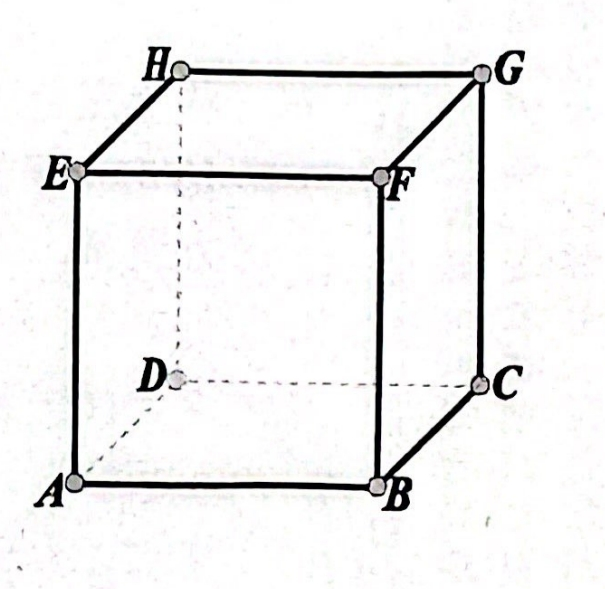
\includegraphics[width=0.2\textwidth]{./pics/Chapter_4/22.png}
%     \end{figure}
%     % 2023.YCB第40届小中组试卷答案.pdf. 8;121
% }